\subsection{Experimental Uncertainties}
\label{sec:ExpSystematics}

\indent Experimental systematics are estimated using a simultaneous fit of CR and the results extrapolated to the SR in a background only fit.  Variations on background yield and kinematics are determined for each systematic by different object performance groups using a number of simulation based and in-situ techniques.  These are variations correspond to the +1 or -1 sigma fluctuation on the gaussian constraint for the systematic.  A simultaneous fit to the CR gives both the background scale factor $\mu$, the best fit value of the systematic parameter $\alpha$, and the systematic uncertainty associated with the background prediction in the SR. \\

\subsubsection*{Uncertainties on the Jet Energy Scale (JES) and Jet Energy Resolution (JER) } 

\indent The two main uncertainties affecting jet measurements are the uncertainties in JES and JER calibrations. The jet reconstruction and calibration process is described in section \ref{sec:reco:jets}.  Uncertainty in the calibration process leads to uncertainty in the calorimeter response to the true jet energy. \\

\indent Since the dominant background, SM ttbar, uses a ttbar control region that requires very similar jet kinematics to the SR, Much of the JES and JER uncertainty is canceled out in the transfer factor between the two.  The JES uncertainty still accounts for one of the major systematic background in the SR at around 10\% in every bin.  Some of this results from extrapolation between the 1L CR and 0L SR where a lepton is effectively replaced with a hadronic tau jet using simulation.  \\

\indent Uncertainties on the JES are derived from different in-situ techniques by the ATLAS Jet/$\met$ group.  These techniques exploit the transverse momentum balance between a jet and a reference object such as a photon or a Z boson or between multiple jets in multijet events.\cite{JES_ZGamma,JES_dijet}.  The uncertainty on JES depends on $\eta$ and $\pt$ of the jet.  Uncertainties related to jet flavor composition and pile-up are also included.  \\

%\indent JES Uncertainty can be parameterized as a combination of 77 nuisance parameters.  This full set of nuisance parameter was combined to give a set of only 4 nuisance parameters.  The distribution of jets showed no dependence on the choice of full or reduced parameter set. \\

\indent The fractional JES uncertainty vs $\eta$ and $\pt$ for 2016 data can be see in figure \ref{fig:sys:JES}. \\

\begin{figure}[!htbp]
\begin{center}
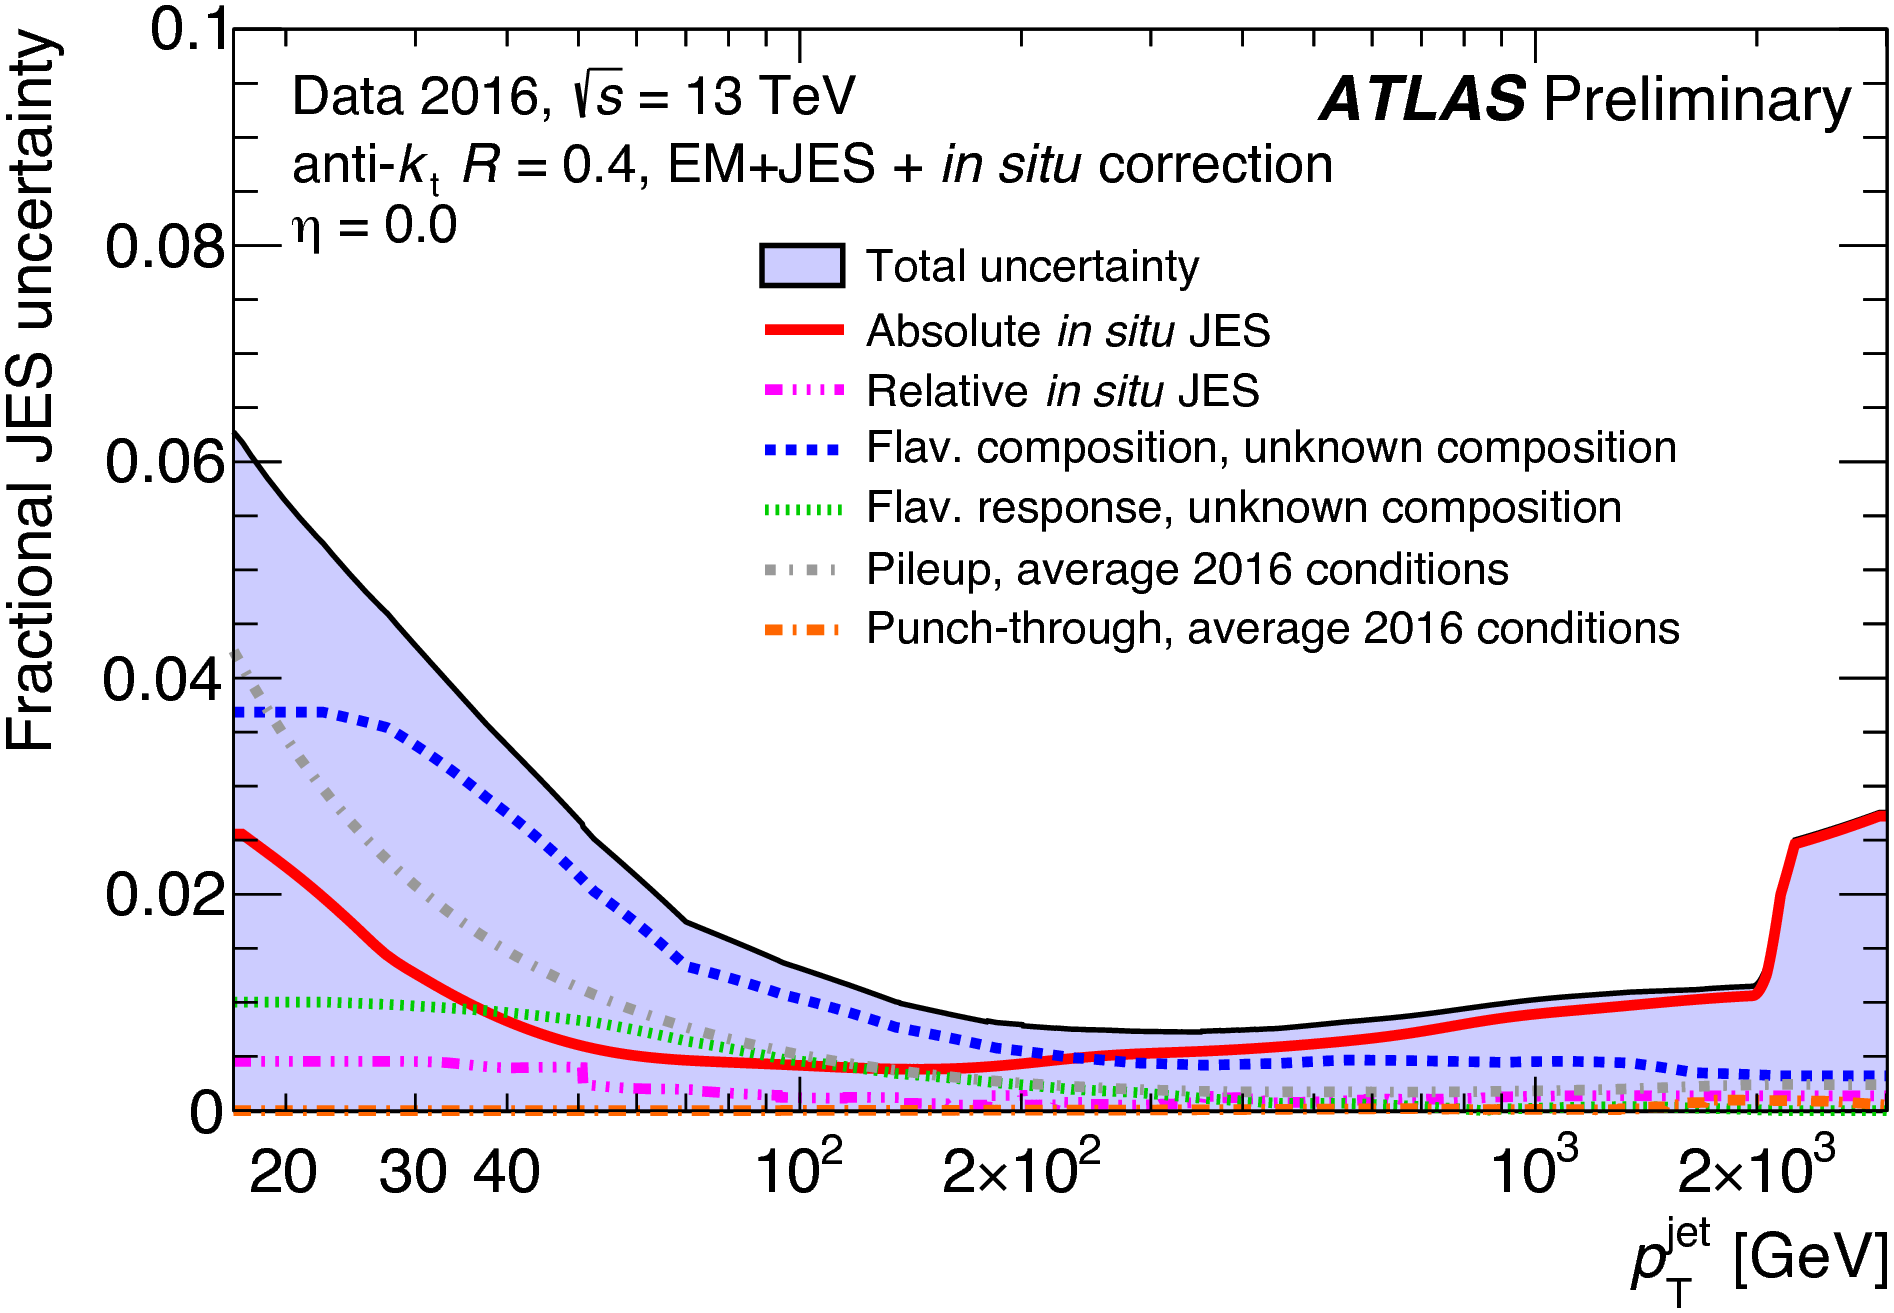
\includegraphics[width=0.48\textwidth]{figures/JetCalib/JES_pt.png}
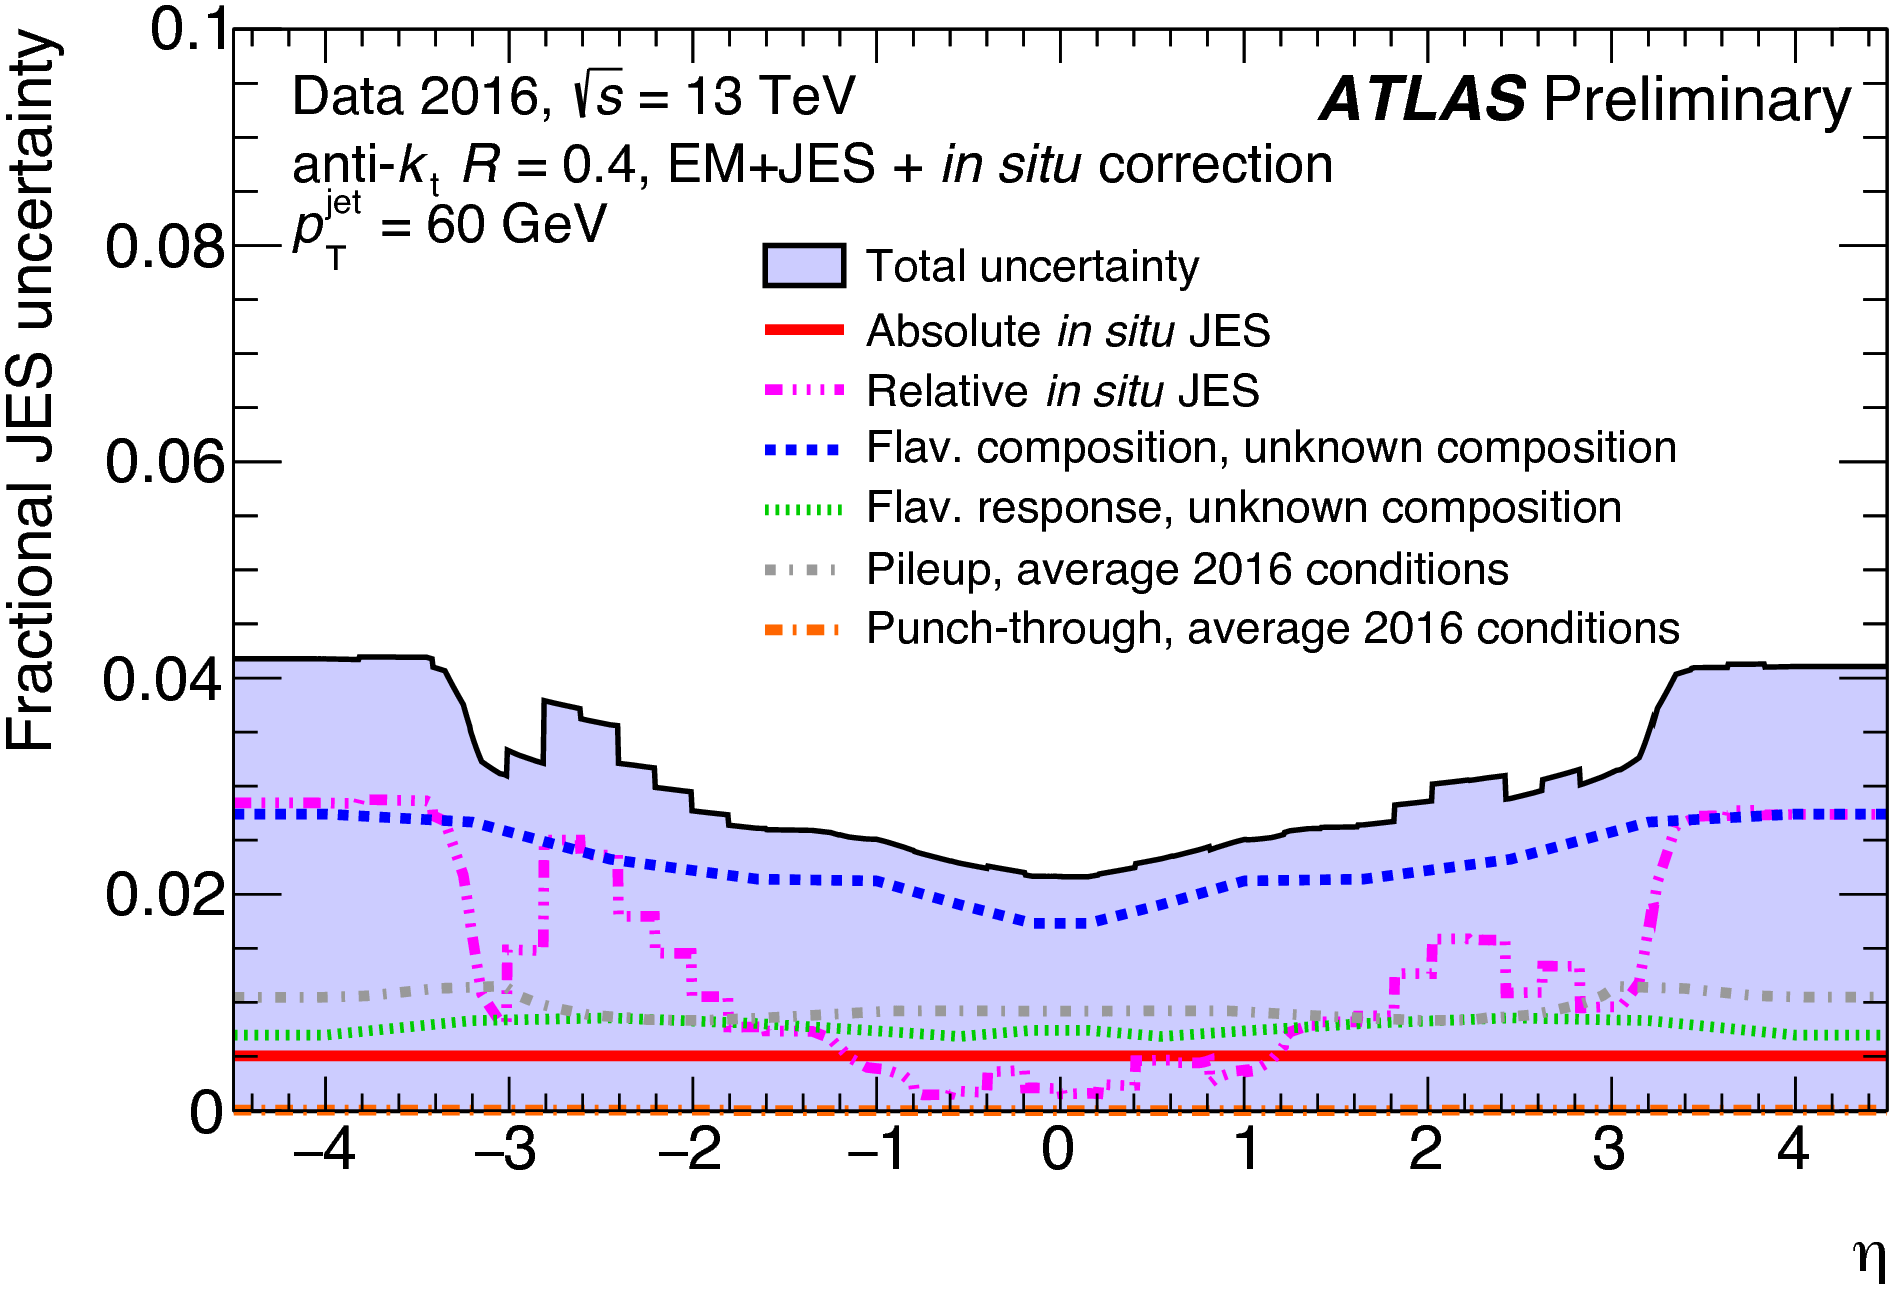
\includegraphics[width=0.48\textwidth]{figures/JetCalib/JES_eta.png}
\caption{Fractional uncertainty on the jet energy scale (JES) vs jet $\eta$ and jet $\pt$.  }
\label{fig:sys:JES}
\end{center}
\end{figure}

\indent Uncertainties on the JER are derived from dijet balance techniques.\cite{JES_dijet}  The fractional uncertainty on JER vs $\eta$ and $\pt$ can be seen in figure \ref{fig:sys:JER}\\

\begin{figure}[!htbp]
\begin{center}
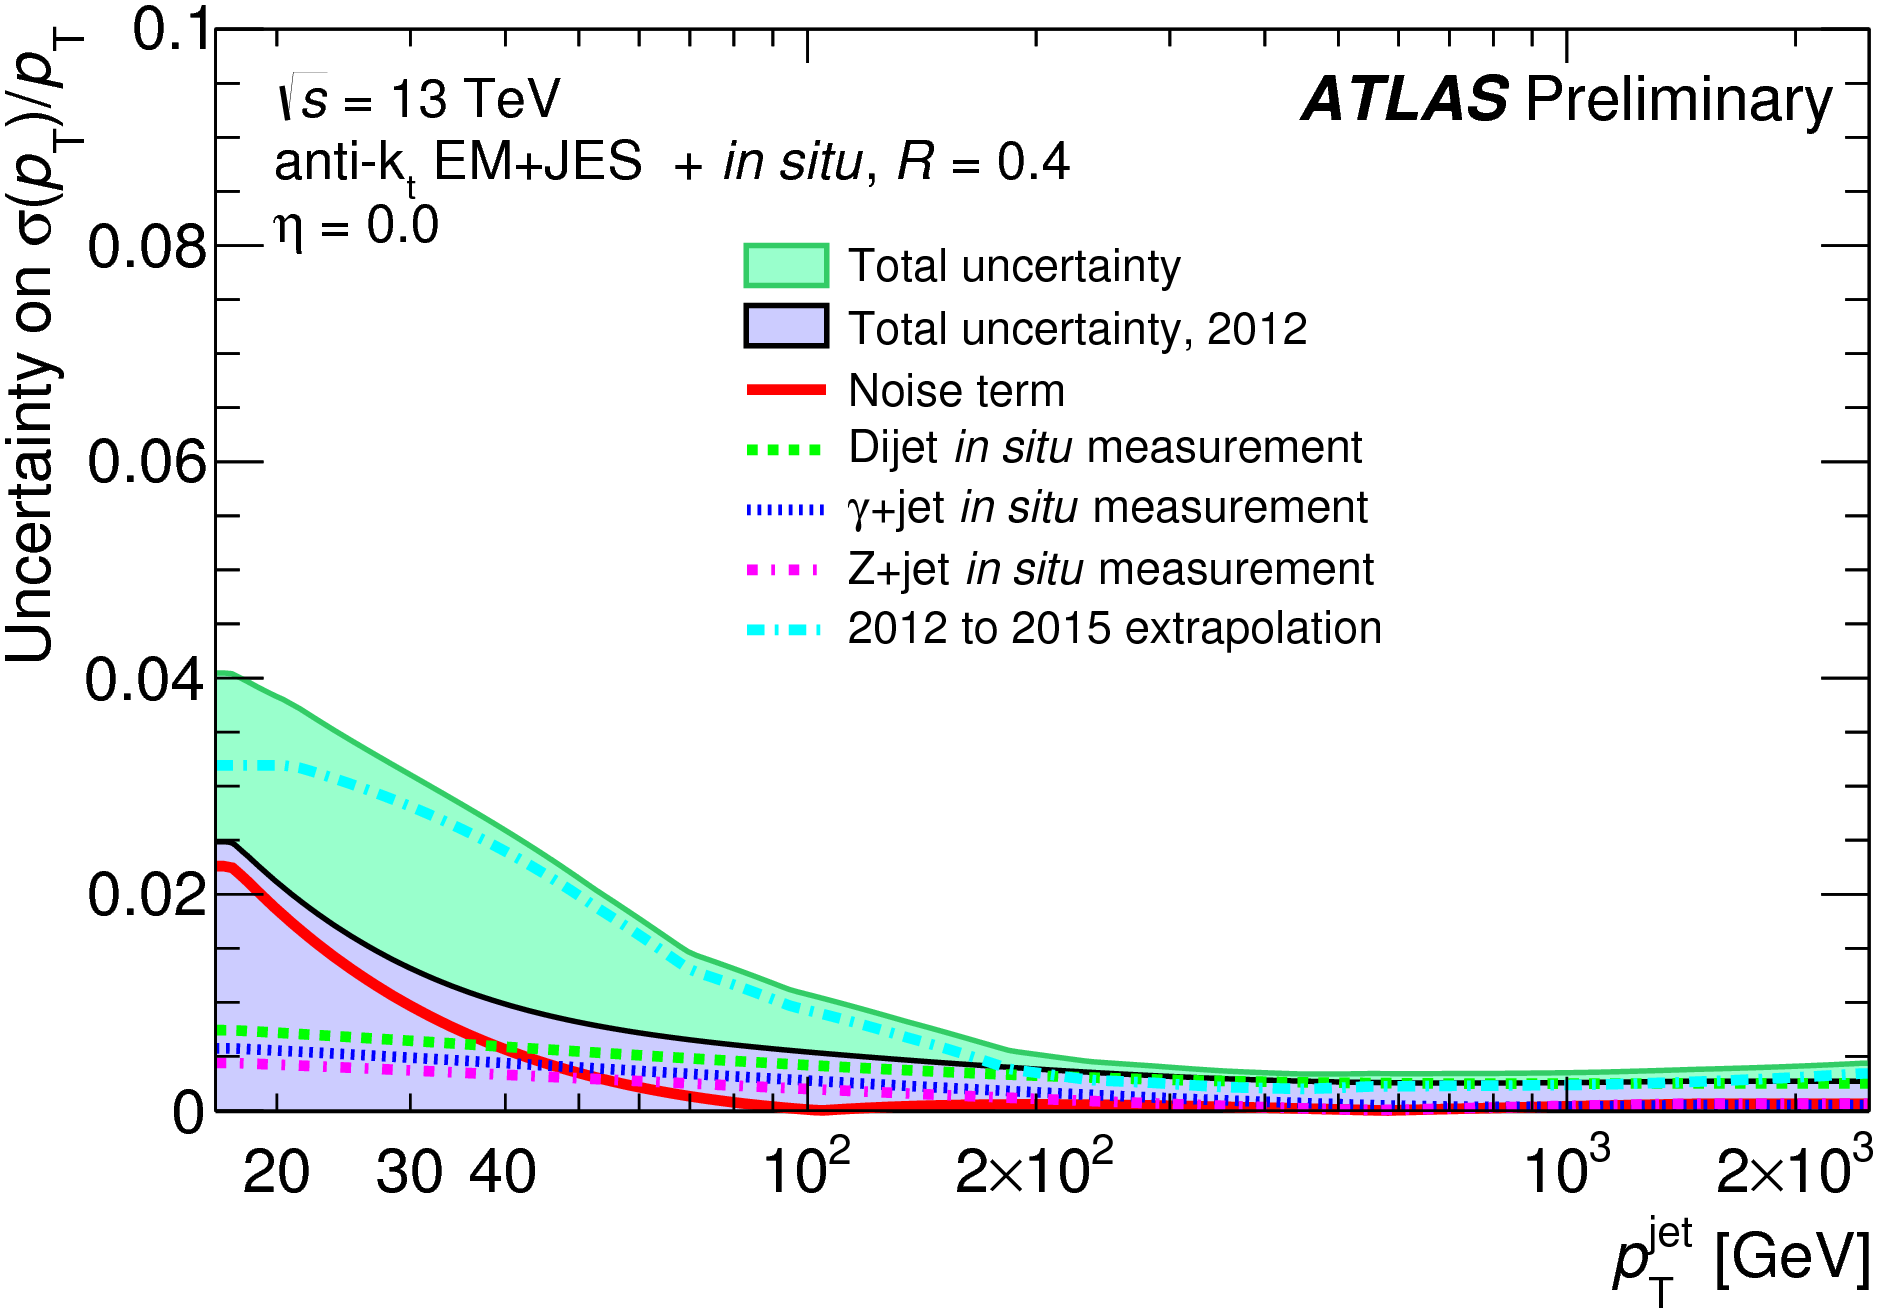
\includegraphics[width=0.48\textwidth]{figures/JetCalib/JER_pt.png}
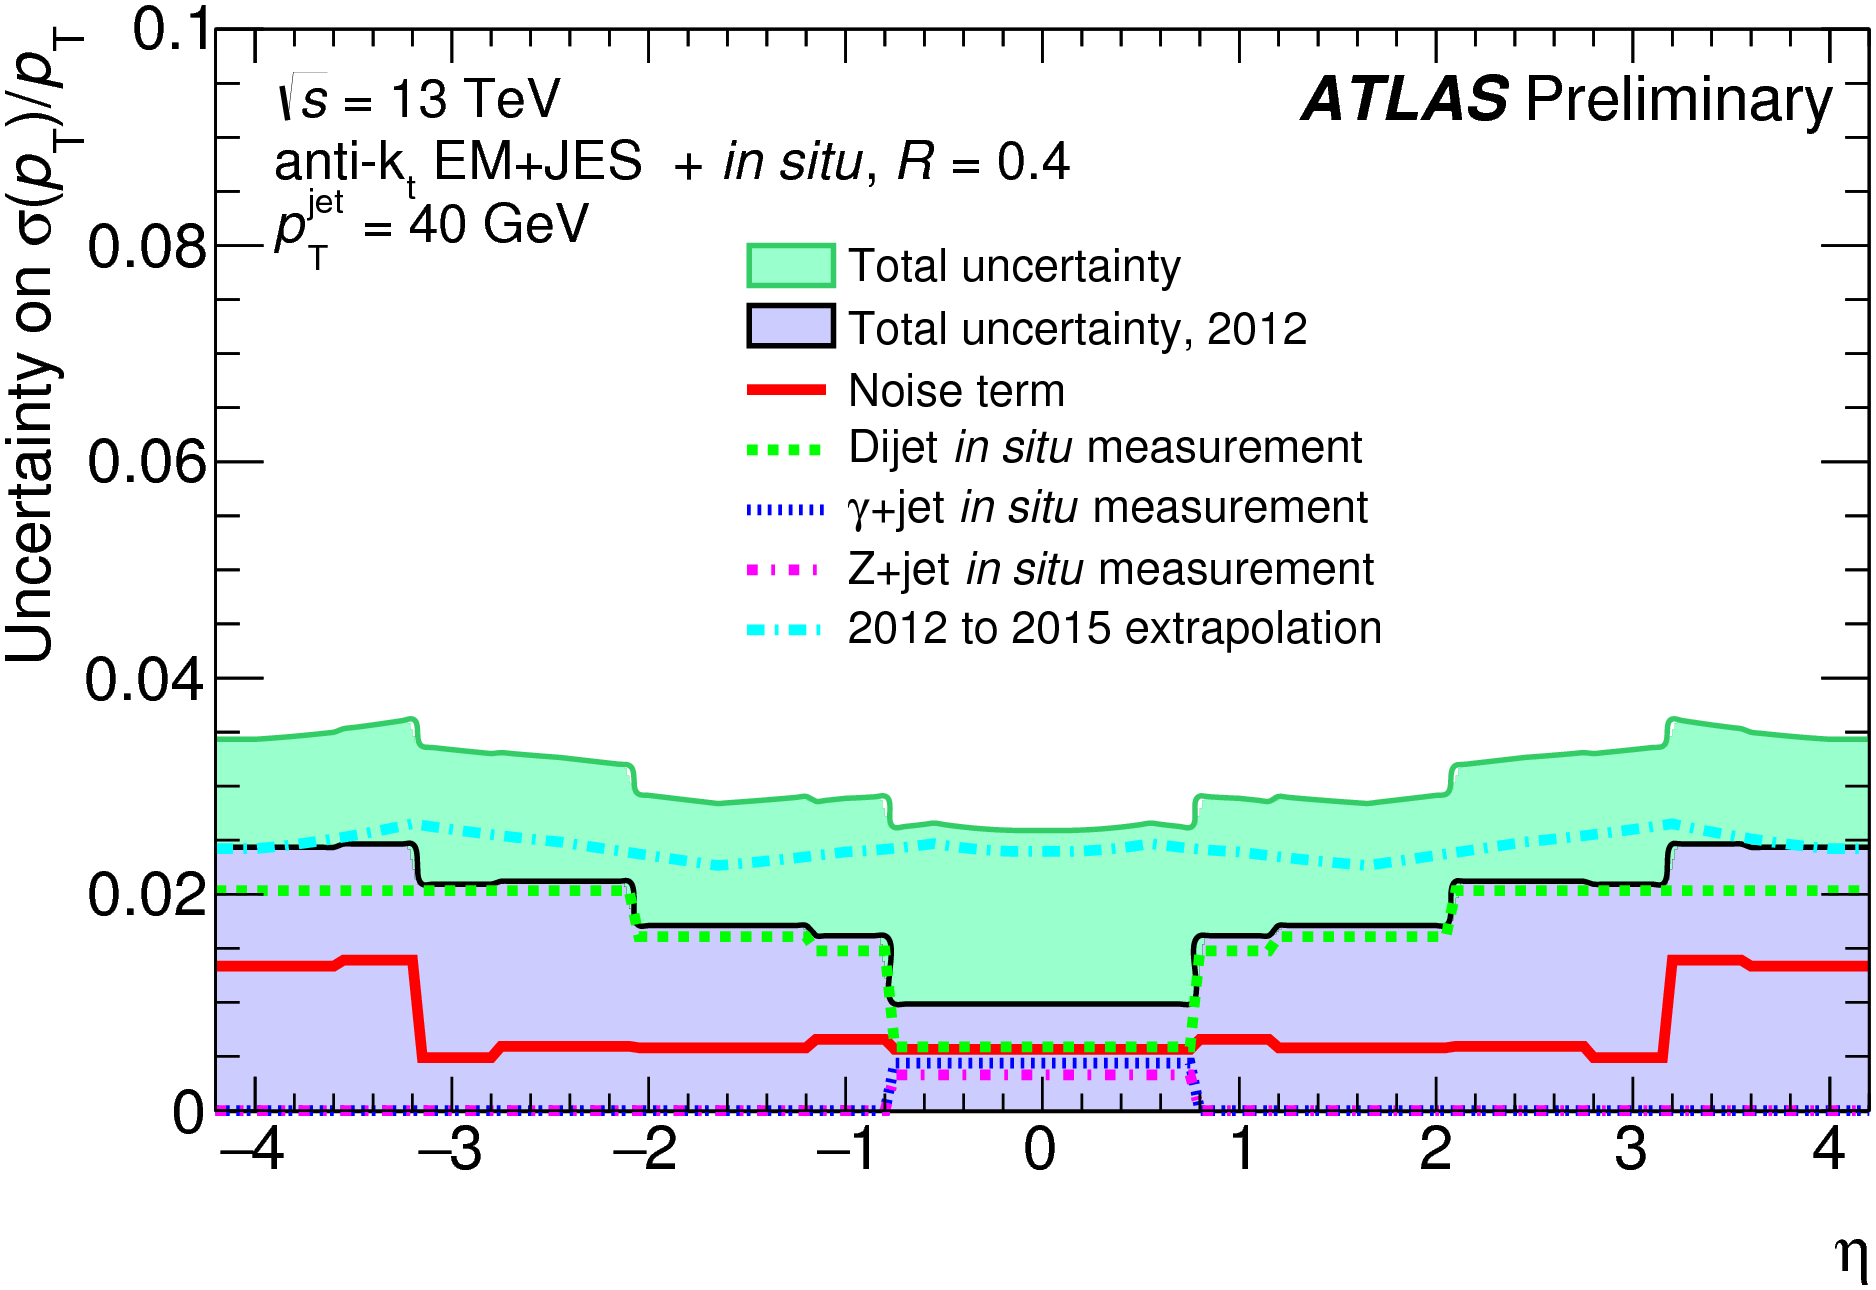
\includegraphics[width=0.48\textwidth]{figures/JetCalib/JER_eta.png}
\caption{Fractional uncertainty on the jet energy resolution (JER) vs jet $\eta$ and jet $\pt$.  }
\label{fig:sys:JES}
\end{center}
\end{figure}

\subsubsection*{Uncertainty on $b$-tagging}

\indent Uncertainties on $b$-tagging are no a large contribution to our systematics due to the fact that we require only a single b-tagged jet and high b-jet $\pt$ requirement of 40 $\gev$.  The dominant background ttbar and sub-dominate backgrounds $W$+jets and QCD multijets all use CRs that also require 1 $b$-tagged jet.  $b$-tagging uncertainty contribute only 1-3\% uncertainty to the total background yield in the SR because of both of these factors.  \\

\indent  The $b$-tagging uncertainty is derived by the ATLAS flavor-tagging working group.  A separate set of weights are applied for each set of $b$-tagging variations.  These include scale factors on $b$-tagging efficiencies and the rate of mis-tagging of $c$-jets and light-flavored jets. \\

\subsubsection*{Uncertainty on the $\met$ Soft Term}

\indent Because the $\met$ is built out of fully calibrated and reconstructed physics objects, the majority of the uncertainty on $\met$ has already been accounted for by jet and lepton momenta and energy uncertainties.  However, the soft term of the $\met$ is the one part of $\met$ reconstruction that does not come from any hard physics object.  The uncertainty on the $\met$ soft term must be estimated independently.  \\

\indent The uncertainty on the resolution and scale of the $\met$ soft term is derived by the ATLAS Jet/$\met$ group using two in-situ methods using $Z\rightarrow \mu\mu$ events. The uncertainty on the $\met$ track soft term (TST) vs the number of reconstructed primary vertexes in $\ttbar$ simulation is shown in figure \ref{fig:sys:MET_TST_tt}. \\

\begin{figure}[!htbp]
\begin{center}
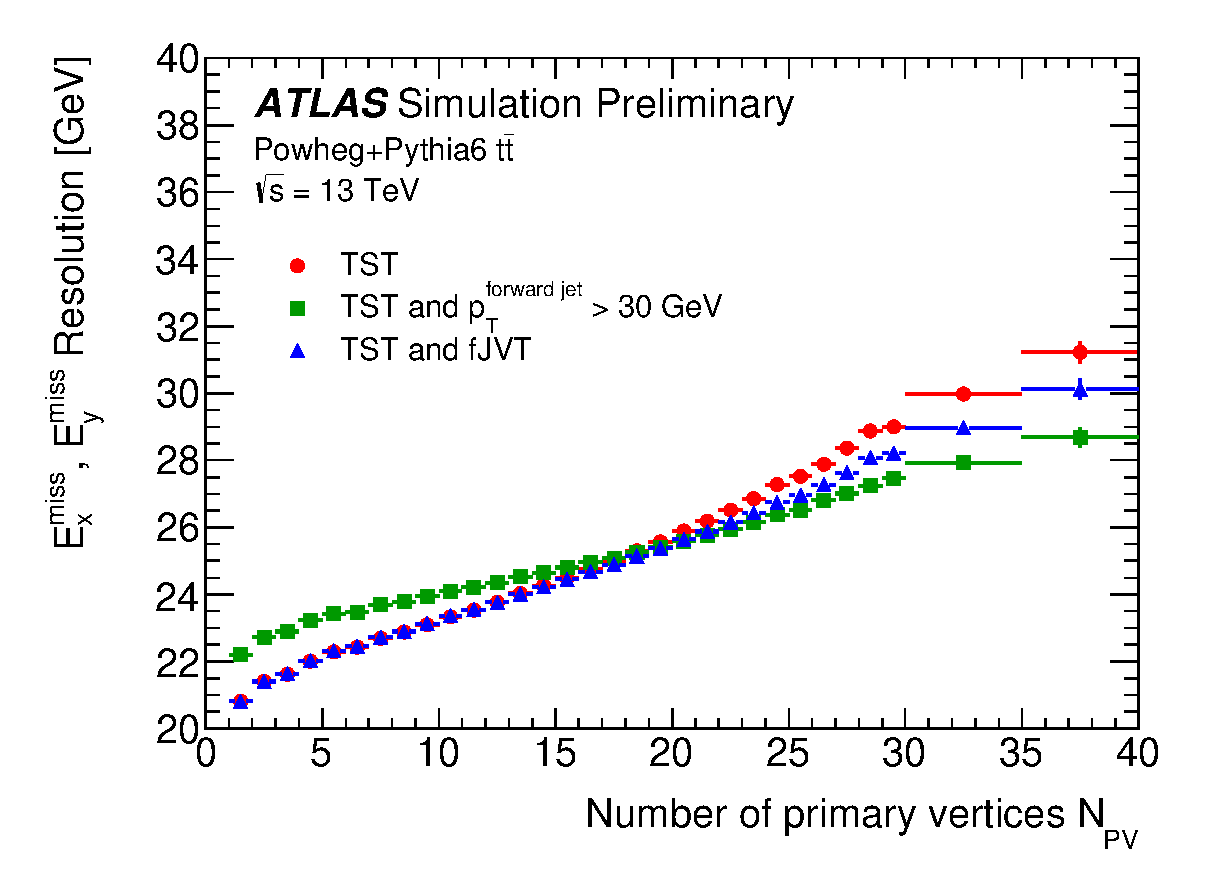
\includegraphics[width=0.48\textwidth]{figures/METCalib/MET_TST_tt.eps}
\caption{Uncertainty on the $\met$ track soft term (TST) vs the number of reconstructed vertexes.  }
\label{fig:sys:MET_TST_tt}
\end{center}
\end{figure}

\indent The $\met$ soft term resolution and scale uncertainty contribute a $1-2\%$ uncertainty on the total background yield.  The small uncertainty result from the high required $\met$ of at least 250 $\gev$ and little to no extrapolation across $\met$ between CR and SR for all major backgrounds. \\

\subsubsection*{Uncertainty on Lepton Reconstruction Efficiencies and Energy Scale}

\indent Uncertainty on lepton reconstruction and identification propagate to uncertainty on CR and SR yields.  These uncertainties include uncertainties on e/$\gamma$ resolution, energy scale, and reconstruction efficiency and muon momenta and reconstruction efficiency.  Lepton trigger scale factors are taken into account for the $\ttbar+\gamma$ control region. \\

\indent These uncertainties are derived by the ATLAS E/$\gamma$ and muon combined performance groups and result in sub 1\% uncertainty on signal region yields. \\

\subsubsection*{Pileup}

\indent The uncertainty on the amount of pileup in 2015 and 2016 ATLAS data is estimated using a two sided variation in event weights.  Pile-up uncertainty contributes a 1-2\% uncertainty on the total background yield in the SR.



  % The detector systematic uncertainties above are calculated as the variations in the shapes of the original normalized histograms using ${\tt overallNormHistoSys}$ inside ${\tt HistFitter}$.
% \item{\bf Luminosity}
%The uncertainty of 2.8 $\%$ is assigned for the integrated luminosity and is denoted by {\bf Lumi} in the fit.


  %%%%%%%%%%%%%%%%%%%%%%%%%%%%%%%%%%%%%%%%%%%%%%%%%%%%%%%%%%
  %% Commented out for the time being since the est, method are not fully defined yet
  %%%%%%%%%%%%%%%%%%%%%%%%%%%%%%%%%%%%%%%%%%%%%%%%%%%%%%%%%%
%% \item{\bf Z fit method for $Z+jets$ background}
%% Following the detailed study in Section~\ref{section:Z_Results}, the uncertainty of 17
%% $\%$ is assigned to $Z+jets$ background for the $Z+jets$ fit-method estimation and is denoted by {\bf methodSysZ} in the fit.

%% \item{\bf Jet-smearing estimation method for multi-jet background}
%% The uncertainty of 100 $\%$ to is conservatively assigned to the
%% multi-jet yields for the jet-smearing estimation method and is denoted by
%% {\bf theoSysQCD} in the fit.

%% \item{\bf \dphimettrk\ and tau veto}
%%   No additional uncertainty is assigned for the requirements on
%%   \dphimettrk\ and on the tau veto. Both were discussed extensively for
%%   the 7 \TeV\ analysis \cite{7TeVSupportNote} where no additional
%%   systematic was assigned.  There are currently no official
%%   recommendations from the jet/etmiss group for \mettrk.  For the 7
%%   \TeV\ analysis, Fig 42 in Appendix C showed good agreement between
%%   data and MC for \dphimettrk\ in the tau-veto-inverted validation
%%   region.  For the current analysis, Fig. \ref{fig:SRA_dataMC} shows
%%   good agreement for the \mettrk\ variables in a \ttbar\ dominated
%%   region.  Tau veto systematics are documented in Appendix D of the 7
%%   \TeV\ note.  Data/MC comparisons were made for several variables in
%%   the 1-lepton control region and in the tau-veto-inverted validation
%%   region.  The tau fake rate was determined in a $Z\nu\nu$+jets
%%   dominated sample to be around 12\%. The systematic on this fake rate
%%   was determined with a study of the track multiplicity in jets; the
%%   track multiplicity for ($n_{trk} \le 4$) showed agreement within 5\%
%%   between data and MC.

  %%%%%%%%%%%%%%%%%%%%%%%%%%%%%%%%%%%%%%%%%%%%%%%%%%%%%%%%%%
  %%%%%%%%%%%%%%%%%%%%%%%%%%%%%%%%%%%%%%%%%%%%%%%%%%%%%%%%%%
  

  
